%----------------------------------------------------------------------------------------
% Analisi del contesto
%----------------------------------------------------------------------------------------

\documentclass[10pt]{softeng} % Document font size and equations flushed left

%----------------------------------------------------------------------------------------
%	ARTICLE INFORMATION
%----------------------------------------------------------------------------------------

\Phase{Inception - I iterazione} % Additional notes (e.g. copyright, DOI, review/research article)

\DocumentTitle{Analisi del contesto e studio di fattibilit\`a} % Article title

%----------------------------------------------------------------------------------------

\begin{document}

\startofdocument{}

% intenzione progetto, collocazione

\section{Fattibilit\`a}

Obiettivo del progetto \`e la realizzazione di un software di Home Banking, i cui utenti sono unicamente persone fisiche.
Un software di Home Banking deve (idealmente) permettere all'utente di effettuare via internet (attraverso un semplice browser web) tutte le operazioni che pu\`o normalmente effettuare allo sportello della sua banca.

Per motivi di sicurezza, legislativi, burocratici e tecnologici non \`e possibile effettuare ogni operazione via internet.
Un sistema di Home Banking effettuer\`a quindi un sottoinsieme proprio di queste operazioni.

Poich\'e l'insieme di operazioni pu\`o essere ridotto arbitrariamente, riteniamo scontata la fattibilit\`a pratica del sistema.
Perch\'e lo sforzo di sviluppo sia ripagato \`e per\`o necessario che l'insieme di operazioni offerte dal sistema sia sufficientemente ampio da:
\begin{enumerate}
	\item soddisfare le esigenze della maggioranza degli utenti;
	\item essere generale al punto da fornire tutti i principali servizi di cui la banca che utilizza il software ha bisogno.
\end{enumerate}
L'effettiva fattibilit\`a viene quindi da una combinazione delle due considerazioni.

Attualmente la quasi totalit\`a banche dispongono di un sistema di Home Banking.
L'introduzione dello standard OBP rende per\`o tutti questi sistemi obsoleti.
Il nostro progetto soddisfa un mercato che avr\`a bisogno in tempi brevi di un nuovo sistema di Home Banking.
Inoltre un software di Home Banking modulare e facilmente personalizzabile pu\`o essere adattato alle esigenze di pi\`u banche con \emph{refactoring} minimo, e quindi a costi ridotti.

% concetti base
\section{Concetti base}

Chiamiamo ``utente registrato (al sistema di Home Banking della banca X)'' una persona fisica titolare di un account di Home Banking all'interno del sistema di una particolare banca, e che quindi abbia fornito informazioni anagrafiche e di contatto, e eventualmente informazioni non obbligatorie sulla sua condizione economica e famigliare.

Chiamiamo ``utente titolare di un conto corrente'' un utente registrato presso la banca X che abbia ultimato la procedura di autenticazione della suddetta banca.

Il bonifico \`e un trasferimento di denaro da un conto corrente a un altro.
Un utente titolare di un conto corrente pu\`o effettuare bonifici dal suo conto corrente.
Distinguiamo due tipi di bonifici:
\begin{itemize}
	\item Bonifico Italia se il conto corrente destinatario \`e aperto presso una banca italiana.
	Per effettuare un Bonifico Italia \`e necessario conoscere nome, cognome, indirizzo e codice IBAN del destinatario.
	\item Bonifico SEPA se il conto corrente destinatario \`e aperto presso una banca europea. Per effettuare un Bonifico SEPA \`e necessario conoscere anche il codice BIC/SWIFT della banca del destinatario \cite{bonifico_unicredit}.
\end{itemize}
Poich\'e la maggioranza dei pagamenti che una persona deve effettuare (tasse, bollette, ricariche, etc.) avvengono tramite bonifico, utenti di un sistema di Home Banking ritengono utile la possibilit\`a di effettuare pagamenti di un certo tipo tramite ``maschere specializzate'', che facilitino la compilazione dei dati e aiutino l'utente a evitare errori.

% Certificati di deposito

% necessit\`a della banca

\section{Portafoglio fondi}

La gestione di un portafoglio fondi \`e un argomento complesso.

% TODO ricontrollare
Le norme che regolano l'acquisto di azioni e le procedure necessarie per acquisire dati aggiornati sull'andamento dei titoli esulano dalla portata di questo progetto, ricadendo nell'area di competenza del \emph{trading online}, e non dell'Home Banking.

\section{Legislazione taliana}

La Banca d'Italia si occupa di esercitare ``l'attivit\`a di vigilanza sulle banche'', e ``ha funzioni di controllo in materia di antiriciclaggio'' \cite[Funzioni]{banca_italia}.

\section{Conclusioni}

Riteniamo sia fattibile, con le limitazioni indicate, realizzare un sistema di Home Banking all'avanguardia, manutenibile, espandibile e generale.

%----------------------------------------------------------------------------------------
%	REFERENCE LIST
%----------------------------------------------------------------------------------------

\printcustombib{}

%----------------------------------------------------------------------------------------
%	FIGURES
%----------------------------------------------------------------------------------------

\begin{figure*}[hbt]
	\centering
	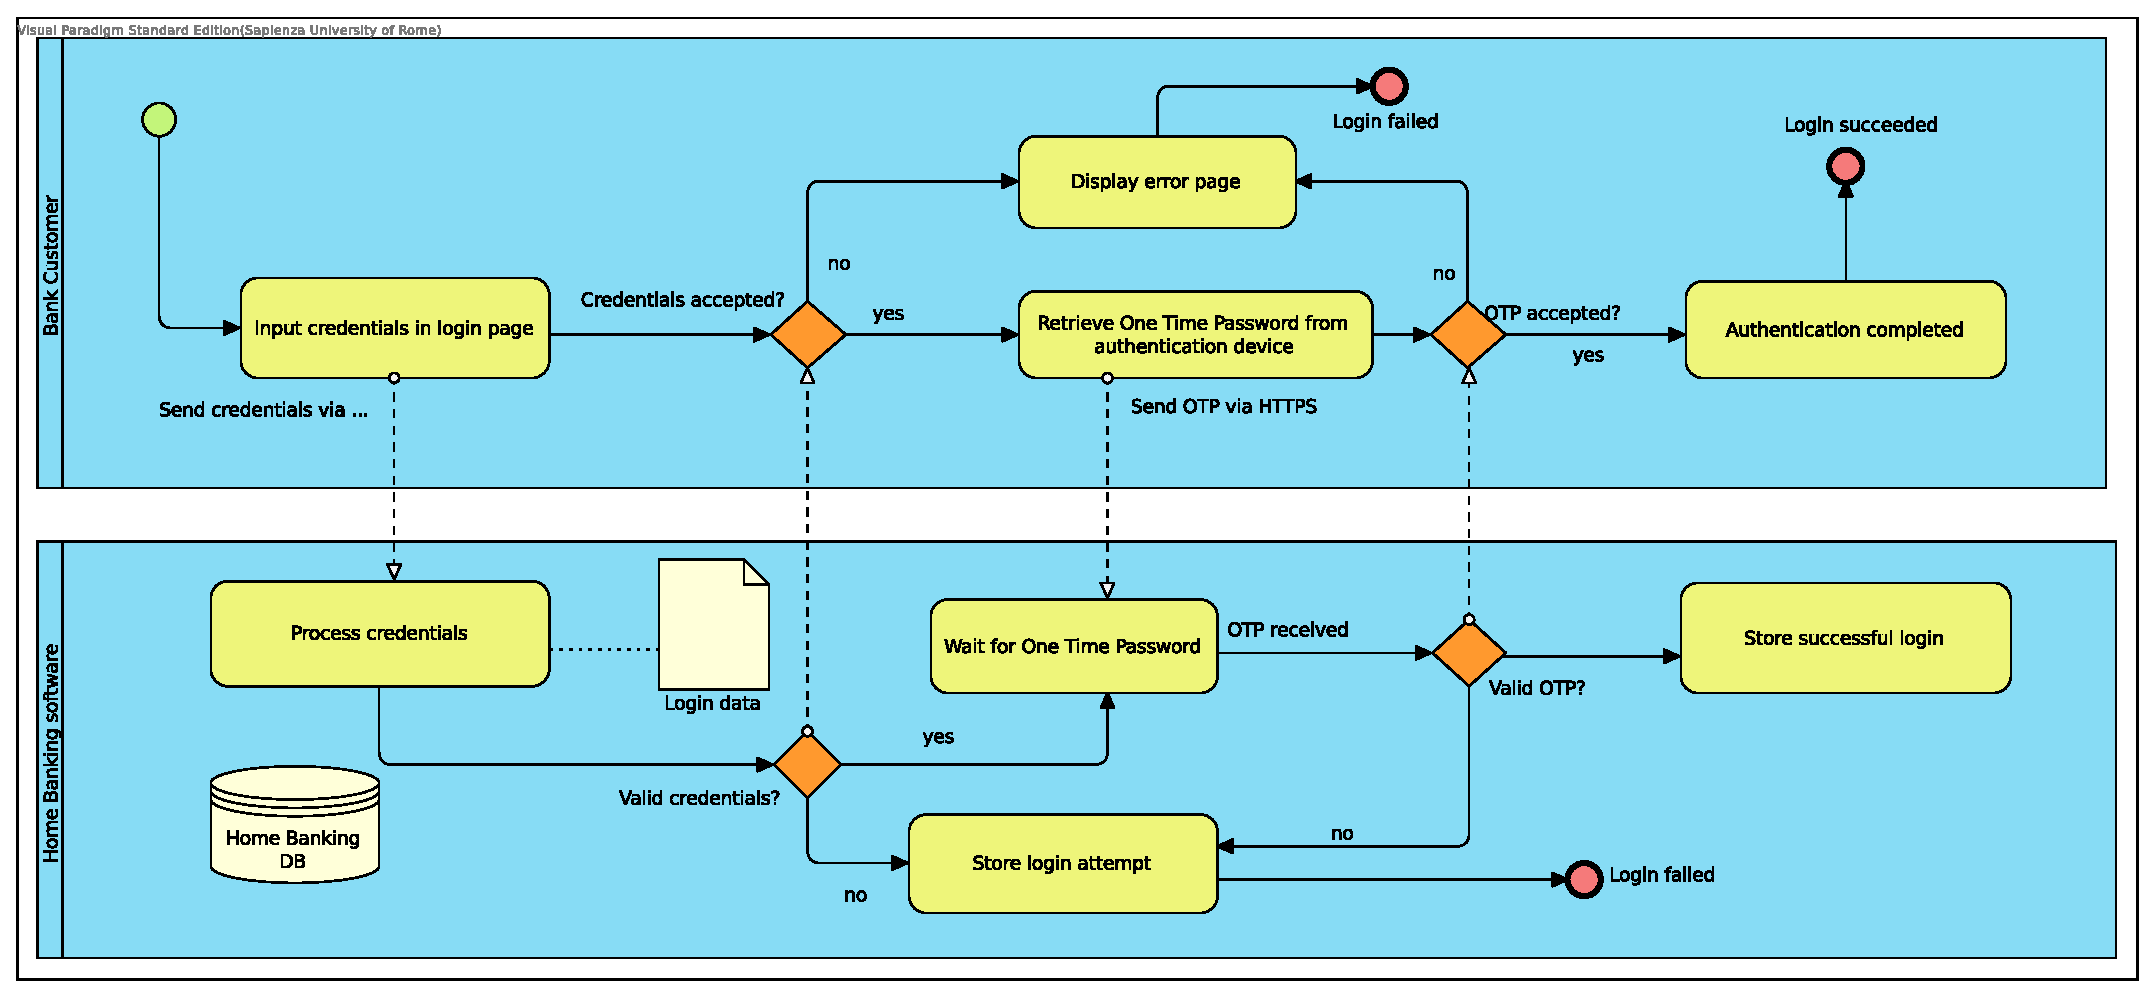
\includegraphics[width=\textheight, angle=90]{Images/Authentication.eps}
	\caption{Business case: procedura di autenticazione.}
	\label{fig:business_case_authentication}
\end{figure*}

\begin{figure*}[hbt]
	\centering
	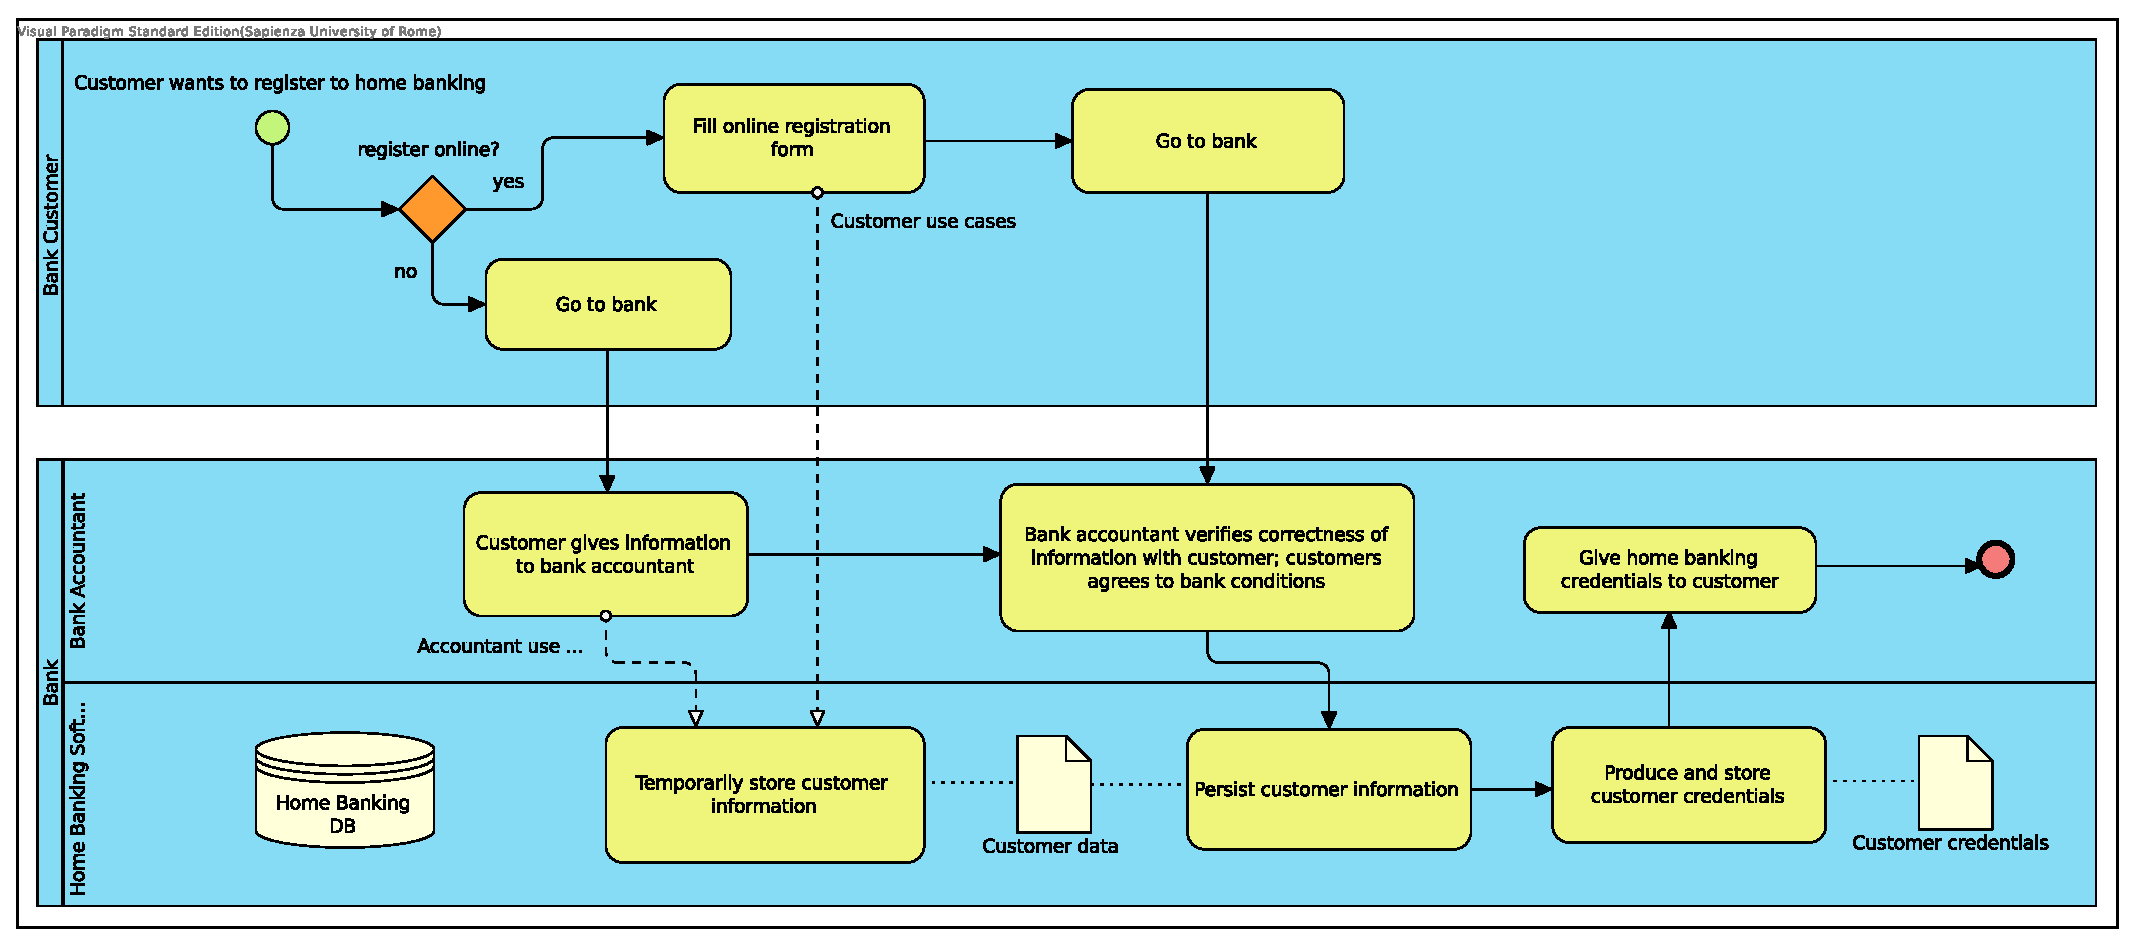
\includegraphics[width=\textheight, angle=90]{Images/Home_Banking_registration.eps}
	\caption{Business case: procedura di autenticazione.}
	\label{fig:business_case_authentication}
\end{figure*}

\end{document}